% topic3.tex -- Module 8 Topic 3: Quantum mechanical nature of the atom, Q29-42.
\topictitle{Topic 3 - Quantum Mechanical Nature of the Atom}

% ---- Q29 (problem with Rutherford's model)
\begin{quizq}{}
Why could Rutherford's model not explain why atoms are stable?
\opts{The nucleus is too small to hold on to the electrons.}
  {In classical physics, orbiting electrons are accelerating, so they would give out electromagnetic
   radiation, lose energy and spiral into the nucleus.}
  {The model did not include neutrons.}{Alpha particles would break the atom apart.}
\end{quizq}

% ---- Q30 (observation explained by Bohr, not Rutherford)
\Needspace{15\baselineskip}
\begin{quizq}{}
Which observation was explained by Bohr's model of the atom, but not by Rutherford's model?
\opts{Hydrogen gas emits light only at certain wavelengths.}
  {Most alpha particles pass straight through a thin gold foil.}
  {Atoms are electrically neutral.}{Cathode rays are deflected by magnetic fields.}
\end{quizq}

% ---- Q31 (Bohr's postulates)
\Needspace{15\baselineskip}
\begin{quizq}{}
Which statement is one of Bohr's postulates?
\opts{Electrons can move in any orbit, and they radiate energy all the time.}
  {The nucleus contains protons and neutrons.}
  {Electrons exist only in certain stationary states, in which they do not radiate energy.}
  {Electrons are spread evenly through a sphere of positive charge.}
\end{quizq}

% ---- Q32 (Rydberg: 3 -> 2)
\Needspace{12\baselineskip}
\begin{quizq}{}
What is the wavelength of the light emitted when the electron in a hydrogen atom moves from $n = 3$ to
$n = 2$?
\opts{\qty{122}{nm}}{\qty{252}{nm}}{\qty{547}{nm}}{\qty{656}{nm}}
\end{quizq}

% ---- Q33 (energy-level diagram: shortest wavelength)
% schematic spacing (not to scale)
\Needspace{28\baselineskip}
\begin{quizq}{}
The diagram shows some of the energy levels of the hydrogen atom (not to scale).
\begin{center}
  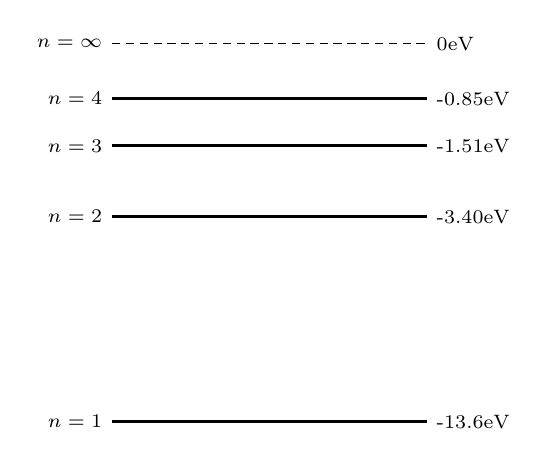
\begin{tikzpicture}
    \foreach \n/\E/\y in {1/-13.6/0, 2/-3.40/2.6, 3/-1.51/3.5, 4/-0.85/4.1} {
      \draw[line width=1pt] (0,\y) -- (4,\y);
      \node[left, font=\scriptsize] at (0,\y) {$n = \n$};
      \node[right, font=\scriptsize] at (4,\y) {\qty{\E}{eV}};}
    \draw[line width=0.6pt, dash pattern=on 3pt off 2pt] (0,4.8) -- (4,4.8);
    \node[left, font=\scriptsize] at (0,4.8) {$n = \infty$}; \node[right, font=\scriptsize] at (4,4.8) {\qty{0}{eV}};
  \end{tikzpicture}
\end{center}
Which transition emits the photon with the shortest wavelength?
\opts{$n = 4$ to $n = 3$}{$n = 2$ to $n = 1$}{$n = 3$ to $n = 2$}{$n = 4$ to $n = 2$}
\end{quizq}

% ---- Q34 (number of lines from n = 4)
\Needspace{12\baselineskip}
\begin{quizq}{}
Hydrogen atoms are excited to the $n = 4$ level. How many different wavelengths can they emit as they
return to the ground state?
\opts{3}{4}{6}{10}
\end{quizq}

% ---- Q35 (absorption: ground state to n = 3)
\Needspace{13\baselineskip}
\begin{quizq}{}
A hydrogen atom in its ground state (\qty{-13.6}{eV}) absorbs a photon and moves to the $n = 3$ level
(\qty{-1.51}{eV}). What is the energy of the photon?
\opts{\qty{13.6}{eV}}{\qty{12.1}{eV}}{\qty{10.2}{eV}}{\qty{1.51}{eV}}
\end{quizq}

% ---- Q36 (de Broglie wavelength of an electron)
\Needspace{12\baselineskip}
\begin{quizq}{}
What is the de Broglie wavelength of an electron moving at \qty{2.0e6}{m.s^{-1}}?
\opts{\qty{3.6e-10}{m}}{\qty{2.0e-13}{m}}{\qty{1.8e-24}{m}}{\qty{1.2e-57}{m}}
\end{quizq}

% ---- Q37 (proton and neutron at the same speed)
\Needspace{16\baselineskip}
\begin{quizq}{}
A proton and a neutron travel at the same speed. How do their de Broglie wavelengths compare?
\opts{The proton's wavelength is much shorter, because the proton is charged.}
  {They are exactly equal, because the particles have the same speed.}
  {The neutron's wavelength is about twice the proton's.}
  {The neutron's wavelength is very slightly shorter, because its mass is slightly larger.}
\end{quizq}

% ---- Q38 (alpha particle and a faster proton)
\Needspace{14\baselineskip}
\begin{quizq}{}
An alpha particle, with about 4 times the mass of a proton, moves at speed $v$. A proton moves at speed
$2v$. How does the de Broglie wavelength of the alpha particle compare with that of the proton?
\opts{It is half as long.}{It is the same.}{It is twice as long.}{It is four times as long.}
\end{quizq}

% ---- Q39 (shortest de Broglie wavelength)
\Needspace{13\baselineskip}
\begin{quizq}{}
Which particle has the shortest de Broglie wavelength?
\opts{An electron moving at \qty{1.0e6}{m.s^{-1}}}{An electron moving at \qty{5.0e6}{m.s^{-1}}}
  {A proton moving at \qty{1.0e3}{m.s^{-1}}}{A proton moving at \qty{2.0e4}{m.s^{-1}}}
\end{quizq}

% ---- Q40 (Davisson-Germer)
\Needspace{15\baselineskip}
\begin{quizq}{}
What did the Davisson--Germer experiment show?
\opts{Electrons have a negative charge.}{Light is made of photons.}
  {Electrons fired at a nickel crystal form a diffraction pattern, so electrons behave as waves.}
  {The nucleus is small and dense.}
\end{quizq}

% ---- Q41 (de Broglie and Bohr's orbits)
\Needspace{16\baselineskip}
\begin{quizq}{}
How did de Broglie's matter waves explain Bohr's stationary states?
\opts{An orbit is stable only if a whole number of electron wavelengths fits around it, forming a
   standing wave.}
  {Electrons orbit the nucleus at the speed of light.}
  {Electron waves cancel out inside the nucleus.}
  {Electrons radiate energy all the time, but very slowly.}
\end{quizq}

% ---- Q42 (limitation of Bohr's model)
\Needspace{16\baselineskip}
\begin{quizq}{}
Which was a limitation of Bohr's model of the atom?
\opts{It could not explain the spectrum of hydrogen.}
  {It could not explain the spectra of atoms with more than one electron, or why some spectral lines
   are brighter than others.}
  {It did not include a nucleus.}{It predicted that atoms are unstable.}
\end{quizq}
